\documentclass[a4paper,12pt,draft]{article}

\usepackage{enumitem}
\usepackage[utf8]{inputenc}
\usepackage{textcomp}
\usepackage{xspace}
\usepackage[italian]{babel}
\usepackage[pdftex,final]{graphicx}
\usepackage{fullpage}
\usepackage{amsmath}
\usepackage{subfig}
\usepackage{multirow}

\usepackage{listings}
\lstset{
	basicstyle=\fontsize{8}{12}\ttfamily,
	inputencoding=utf8,
	language=Java,
	numbers=left,
	numberstyle=\tiny,
	tabsize=2,
	frame=single,
	backgroundcolor=\color{gray},
}


\setenumerate[2]{label=\alph*.}

\usepackage{color}
\definecolor{gray}{gray}{0.9}

\usepackage[final]{hyperref}
\hypersetup{
	colorlinks=true
}
\usepackage{hypcap}

\newcommand{\ddbp}{$2D -$\emph{bin packing}}
\newcommand{\ddbpp}{problema \ddbp{}}

\begin{document}

\thispagestyle{empty}
\begin{center}
	\leavevmode
	\large
	\begin{tabular}{ r l }
		\multirow{2}{*}{
\includegraphics[width=2cm]{img/unipd_logo.png}} & \textsc{Università degli studi di Padova}\par \\
			& \textsc{Corso di laurea magistrale in Ingegneria Informatica} \\
	\end{tabular}
	\vskip 3cm
	
	\vfill
	\textbf{{\large Relazione del progetto del corso di Intelligenza Artificiale}}\\[0.2cm]
	\textbf{{\LARGE Approcci metaeuristici al 2D Bin Packing Problem}}\par
	\vskip 3cm
	\normalfont
	
	\begin{tabular}{ c c c }
		\large Luca \textsc{Gasparini} & Alberto \textsc{Boccato} &
				Nicola \textsc{Chessa} \\
		\normalsize 999999 & 999999 & 1014413 \\
	\end{tabular}
	\vskip 0.5cm
	\begin{tabular}{ c c }
		\large Nicola \textsc{Dalla Benetta} & Nicola \textsc{Gobbo} \\
		\normalsize 1020097 & 1014195 \\
	\end{tabular}
	\normalfont
	\vskip 4cm
	
	\begin{flushright}
		\emph{Docente:}\\
		Prof. Silvana \textsc{Badaloni}\\
	 \vskip 2cm
		\emph{Collaboratori:}\\
		Dott. Francesco \textsc{Sambo}\\
	\end{flushright}

	
	\vfill
	{\large A.A. 2011-2012}
\end{center}
\cleardoublepage


\begingroup
	\hypersetup{linkcolor=black}
	\setcounter{tocdepth}{2}
	\tableofcontents
\endgroup

\newpage

\section{Introduzione}
Lo scopo di tale relazione è quello di illustrare alcuni algoritmi
metaeuristici per risolvere il problema del 2D Bin Packing; in particolare
attraverso l'euristica Bottom-Left-Fill (BLF) si sono scelti i seguenti:
\begin{itemize}
\item Genetico;
\item Genetico basato su torneo
\item Tabu Search.
\end{itemize}
Inoltre si è realizzata l'interfaccia grafica per ottere un supporto che
evidenziasse il comportamento di tali algoritmi.

\subsection{Descrizione del problema}
Il 2-D Bin Packing Problem (2-DBPP) con rotazioni è definito come
segue: 
\begin{itemize}
\item dato un insieme di n oggetti rettangolari di dimensioni h_{i} e w_{i}
che rappresentano rispettivamente l'altezza e la larghezza dell’oggetto
i-esimo;
\item dato un insieme illimitato di contenitori, ognuno dei quali ha altezza
H e larghezza W;
\end{itemize}
Minimizzare il numero dei contenitori (nBin) utilizzati a seguito
dell'inserimento di tutti gli oggetti senza sovrapposizione (nBIN) è
l'obbiettivo del problema. Gli oggetti possono essere ruotati di 90 gradi,
questo aumenta le dimensioni dello spazio di ricerca e quindi la difficolta’ per
raggiungere la soluzione ottima, ma produce il vantaggio di ridurre il numero di
contenitori necessari.
I vincoli cui devono sottostare gli algoritmi risolutivi sono i seguenti:
\begin{itemize}
 \item ogni oggetto deve essere inserito in un solo bin;
 \item le dimensioni di ogni singolo oggetto devono essere minori delle
dimensioni del bin;
 \item le dimensioni dell'area totale occupata dalla somma degli oggetti in un
bin deve essere inferiore all'area del bin.
\end{itemize}
Tali vincoli sono necessari altrimenti la soluzione del problema è triviale,
infatti il problema non avrebbe alcuna soluzione.

\subsection{Descrizione generale di un algoritmo per 2-DBPP}
Ogni algoritmo utilizzato in questa relazione ha la seguente struttura.

INPUT:
\begin{itemize}
  \item H e W dimensioni di tutti i bin;
  \item h_{i} e w_{i} dimensioni dell’oggetto i-esimo;
\end{itemize}

OUTPUT:
\begin{itemize}
 \item nBIN numero di bin necessari per contenere gli oggetti;
 \item posizionamento degli oggetti in ogni bin con rappresentazione grafica;
 \item numero delle soluzioni ottime;
 \item tempo di esecuzione;
\end{itemize}

Il 2-DBPP è un problema NP-Completo, ovvero fa parte di quella classe di
problemi per i quali non è possibile, in tempo polimoniale, ottenere una o più
soluzioni ottime.
Proprio da questo aspetto nasce l'esigenza di ottenere buone soluzioni
approssimate che siano ragionevolmente vicine all'ottimo; tali soluzioni si
possono ottenere attraverso la coniugazione di euristiche particolari e
algoritmi metaeuristici. 

\cite{lmvTabu}

\section{Framework di esecuzione}
Il programma sviluppato è stato progettato con l'obiettivo di fornire un framework di esecuzione per algoritmi che risolvono il \ddbpp. L'intento è creare un ambiente in cui, lo sviluppatore che voglia verificare le performance di un nuovo algoritmo, possa concentrarsi solo sullo sviluppo dello stesso, senza preoccuparsi di tutte le problematiche relative alla grafica o alla \emph{user experience}.

\subsection{Aspetto}
Ad un utente finale l'interfaccia grafica si presenta come in figura \ref{fig:main_window_ss}. Da questa finestra è possibile configurare le specifiche del problema quale dimensione dei contenitori, o \emph{bin}, e il numero di pacchetti, o \emph{packet}, con relative larghezze e altezze. Una volta configurato il problema, si potrà scegliere l'algoritmo, o \emph{Core}, con il quale risolverlo: ogni metodo risolutivo ha parametri di configurazione propri, mostrati nella sezione loro dedicata, che possono venir usati per adattare il comportamento dell'algoritmo alla specifica istanza. Una volta completata la fase di configurazione il \emph{Core} può essere lanciato e, ad ogni ottimo trovato, ne verrà visualizzato il \emph{placing}, il valore di fitness, il numero di iterazioni e il tempo impiegato per raggiungerlo.

\begin{figure}[h!tp]
 \centering
 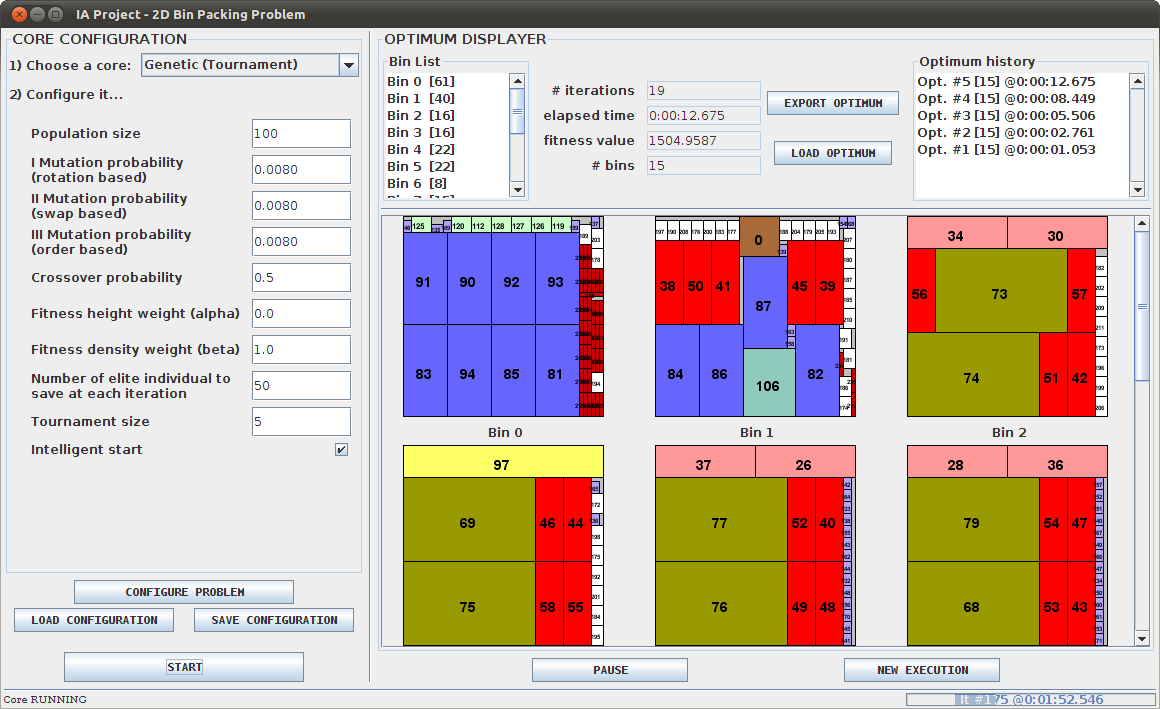
\includegraphics[width=\textwidth]{./img/main_window_ss.png}
 % main_window_ss.png: 1160x709 pixel, 72dpi, 40.92x25.01 cm, bb=0 0 1160 709
 \caption{Screenshot della finestra principale del programma}
 \label{fig:main_window_ss}
\end{figure}

\subsection{Caratteristiche peculiari}
Il framework sviluppato mette a disposizione diverse caratteristiche per facilitare l'utente finale nell'uso del software, così come lo sviluppatore nel test degli algoritmi.
\paragraph{Salvataggio \& caricamento della configurazione corrente}
Attraverso i pulsanti \texttt{SAVE} e \texttt{LOAD CONFIGURATION} è possibile salvare o caricare da file la configurazione del problema attualmente in esame, comprensiva del core selezionato e dei suoi parametri specifici. Il file prodotto sarà formattato secondo lo standard XML e modificabile anche al di fuori del programma.
\paragraph{Cronologia degli ottimi}
Ogni volta che l'algoritmo individua un nuovo ottimo la sua rappresentazione prende il posto della precedente. Questo comportamento può non essere sempre gradito in quanto uno sviluppatore potrebbe voler vedere l'intera evoluzione degli ottimi, per capire se l'algoritmo scritto si comporta nel modo correto, mentre un utente potrebbe accorgersi che, per una non precisa calibrazione della funzione di fitness, un ottimo precedente risulta ``più adatto agli scopi'' di quello successivo. Per porre rimedio a questo ostacolo il framework salva l'intera cronologia degli ottimi che possono così essere visualizzati nuovamente.
\paragraph{Salvataggio \& caricamento di ottimi}
I pulsanti \texttt{EXPORT} e \texttt{LOAD OPTIMUM} permettono all'utente di salvare qualsiasi ottimo presente nella cronologia, nonchè visualizzarlo nuovamente in futuro. Il file prodotto contiene la sequenza di bin con il \emph{placing} dei relativi pacchetti e, essendo in formato XML, può essere facilmente interpretato da un programma di terze parti.
\paragraph{Ingrandimento automatico dei \emph{bin}}
Da un punto di vista esclusivamente di \emph{user experience} la rappresentazione grafica dei \emph{bin} viene riscalata ogni volta che le dimensioni della finestra, e dei \emph{bin} stessi, lo permettono. Ciò facilita l'analisi dell'ottimo trovato soprattutto quando questo è composto da oggetti di piccole dimensioni.

\subsection{Classi essenziali}
L'aggiunta di nuovi \emph{Core} da parte di uno sviluppatore comincia con la comprensione dello schema UML presentato in figura \ref{fig:uml_classi}.
\begin{description}
	\item[\texttt{MainWindow}]
	\item[\texttt{ProblemConfiguration}] La creazione e gestione di questa classe è demandata 
	\item[\texttt{GUISignaler}]
	\item[\texttt{OptimumPainter}]
	\item[\texttt{CoreDescriptor}]
	\item[\texttt{CoreController}]
	\item[\texttt{AbstractCore \& SwingWorker}]
	\item[\texttt{AbstractConfigurator}]
\end{description}


\begin{figure}[h!tp]
 \centering
 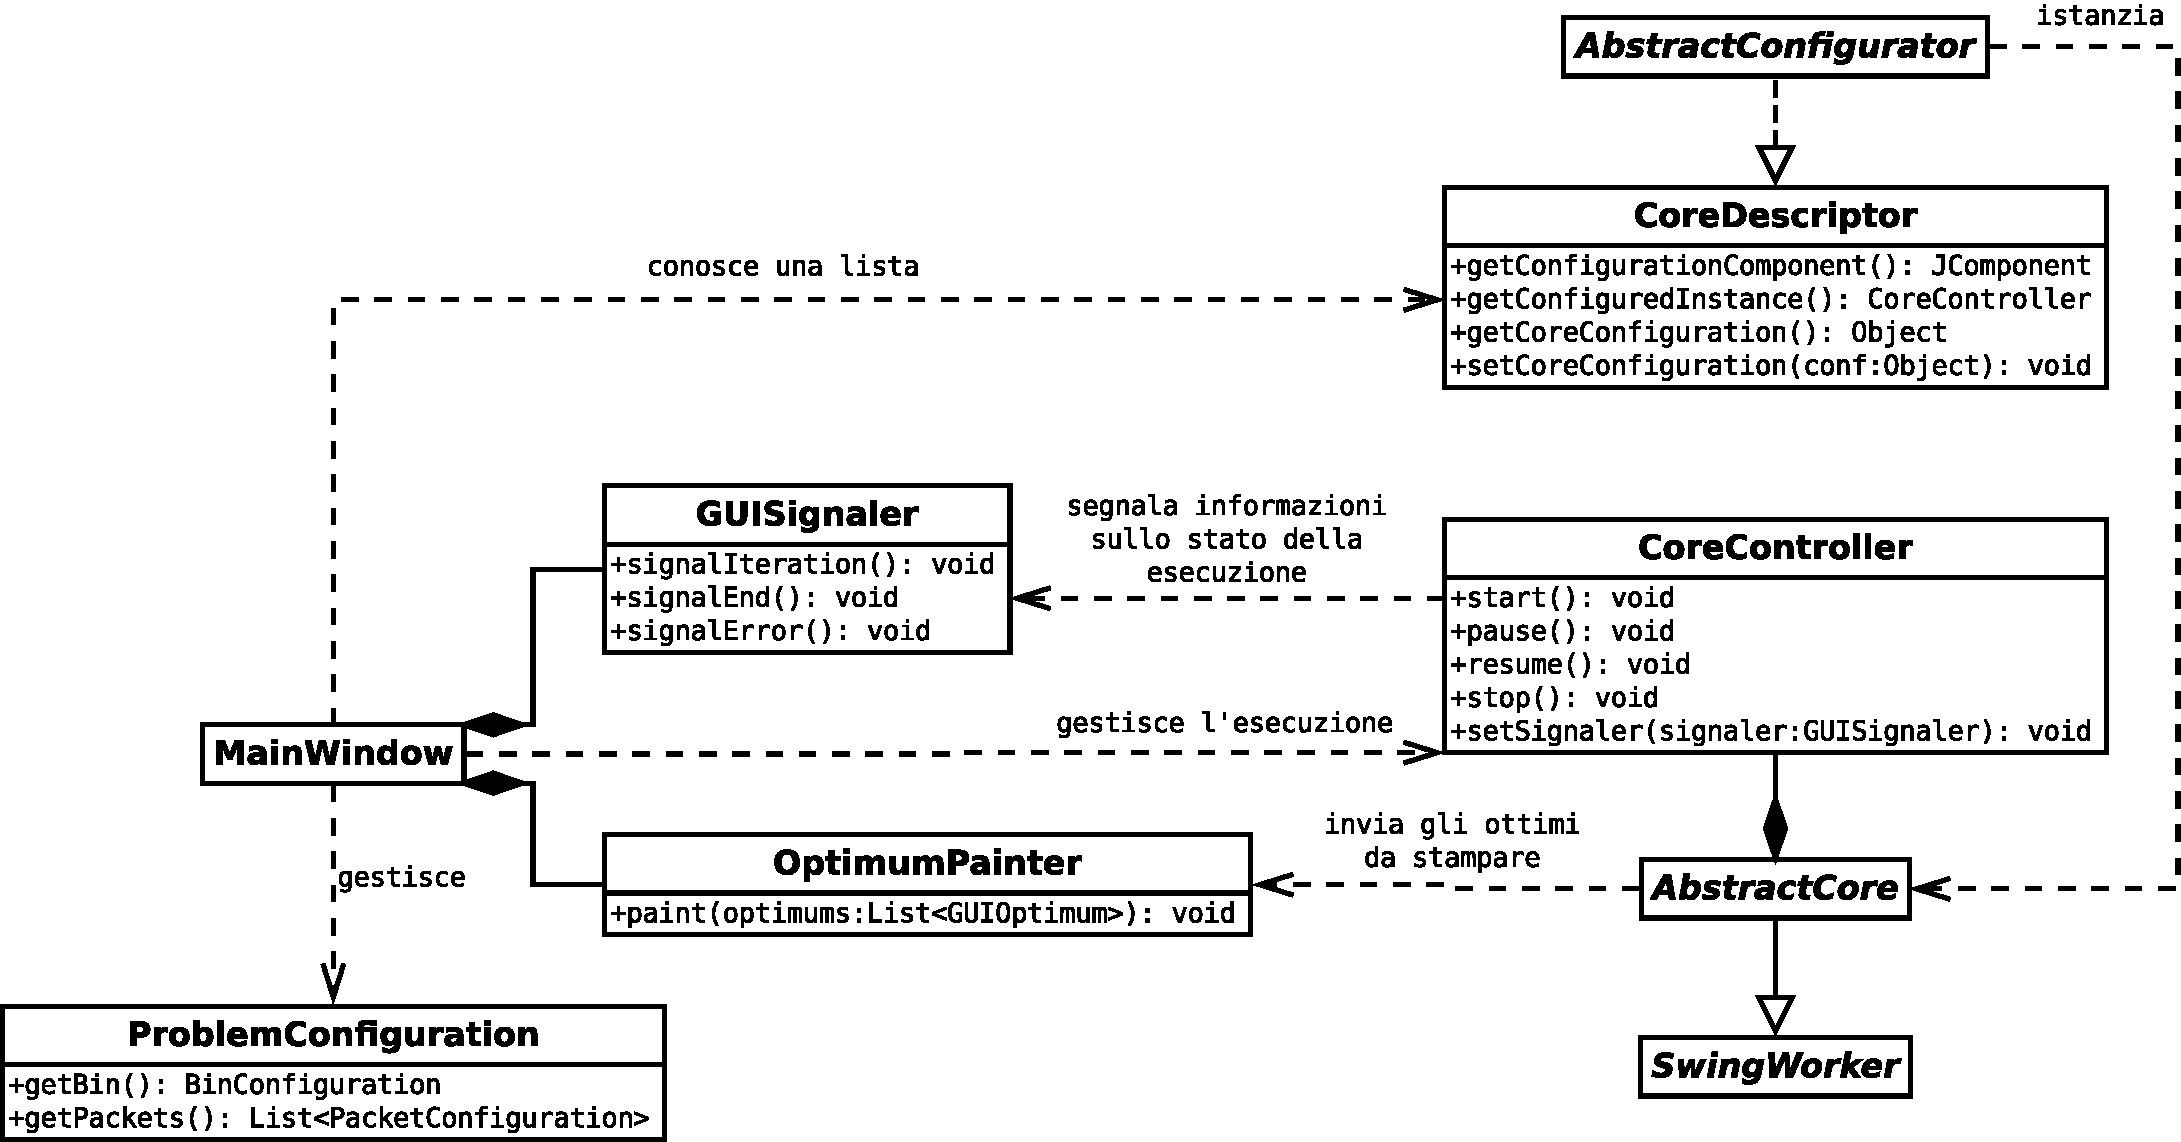
\includegraphics[width=\textwidth]{./img/uml_classi.pdf}
 % uml_classi.pdf: 1047x548 pixel, 72dpi, 36.94x19.33 cm, bb=0 0 1047 548
 \caption{Grafico UML delle classi principali dell'applicazione}
 \label{fig:uml_classi}
\end{figure}


\section{Conclusione}
Dall'esperienza accumulata sviluppando questo progetto è stato valutato che gli algoritmi metaeuristici, nella fattispecie \emph{genetico} e \emph{tabu search}, si comportano bene nella soluzione del \ddbpp. Osservando gli ottimi proposti si nota che in poco tempo ci sono ``andati molto vicini'' seppure si notano comunque possibili margini di miglioramento. Pensando in un ottica di applicazione commerciale questo comportamento è favorevole in quanto risulta più facile ottimizzare un problema partendo già da una soluzione sub-ottima che in poco tempo è riuscita ad individuare pattern particolari.

Confrontando i due \emph{Core} a nostra disposizione la prima differenza che salta all'occhio è nel numero di paramentri: l'algoritmo \emph{genetico} richiede una configurazione più ampia che cambia da un'istanza all'altra, mentre il \emph{tabu search} offre parametri con validità più generale. Detto ciò il \emph{tabu search} risulta essere più intuitivo per la logica umana mentre il \emph{genetico} sembra più casuale nella sua evoluzione ma, dai test effettuati, risulta comportarsi meglio su istanze che coinvolgono pochi bin mentre i due algoritmi tendono a produrre soluzioni equivalenti con l'aumentare del numero di bin necessari.

In rete è possibile trovare programmi commerciali\footnote{In particolare abbiamo individuato il programma \emph{2D Load Packer} della Astrokettle Algorithms (\url{http://www.astrokettle.com/pr2dlp.html}) che forniva una libreria di istanze risolte, usate come metrica di riferimento.} che risolvono il problema del \ddbp, si è deciso quindi di confrontarsi con tali programmi su medesime istanze per valutare la bontà del codice prodotto, è emerso che per quasi tutte le istanze i risultati da noi ottenuti sono molti vicini a quelli ottenibili con i software commerciali. Questo evidenzia il fatto che con particolari accorgimenti potrebbe esser possibile migliorare leggermente quanto ottenuto, le tipologie di algoritmi per problemi quali il \ddbp sono infatti molto sensibili a particolari accorgimenti come ordinamenti o euristiche distinte adottate.

Il programma sviluppato è distribuito sotto licenza GNU GPLv3\footnote{\url{http://www.gnu.org/licenses/gpl.html}} e liberamente scaricabile dal sito \url{https://code.google.com/p/iaproject-2dbpp/}.


\phantomsection
\addcontentsline{toc}{section}{Bibliografia}
\bibliographystyle{plain}
\bibliography{IABibliography}

\end{document}
